\documentclass[10pt,conference]{IEEEtran}

\usepackage[]{hyperref}
\usepackage[]{graphicx}
\usepackage[]{authblk}
\usepackage{multirow}
\usepackage{multicol}

\begin{document}
\title{Miniproject 2 Report}
\author[1]{Olivier Cloux}
\affil[1]{Department of Computer Science, EPFL}

\maketitle

\begin{abstract}
content
\end{abstract}

\section{Introduction}
The emergence of Deep Learning frameworks such as PyTorch \cite{noauthor_pytorch_nodate} or TensorFlow \cite{noauthor_tensorflow_nodate} has allowed for easy developments of ever increasing complexity. But constantly using these hides the true mechanisms behind deep learning. This is why in this report we will try and re-implement a basic deep learning framework for ourselves, to delve into how such a framework works.
\section{Task}
There are two tasks here. The first one, ``front one'' is to build a model to classify binary points, according to their position in the plane. The second, ``actual one'' is to do the other task without using the niceties of PyTorch or other deep learning frameworks, in particular without the \texttt{torch.nn} module.

\subsection{Classification}
Let's talk briefly about the underlying task. It's quite simple: we generate $N$ random points in the $[0,1]^2$ square, and then assign a label of 1 to all points inside the $1/\sqrt{2\pi}$ circle, and 0 outside.
\begin{figure}[h]
    \centering
    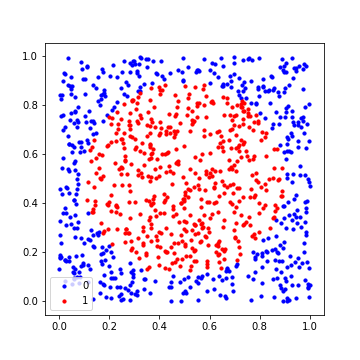
\includegraphics[scale=0.5]{../images/dataset.png}
    \caption{A 1000-points dataset}
    \label{fig:dataset}
\end{figure}
Figure \ref{fig:dataset} shows an instance of such dataset.
\section{Framework}
The framework I created follows the general idea of PyTorch but allows for more flexibility. It is split in 3 files:
\subsection{modules.py}
This file contains a meta class \texttt{Module}, and all other classes inherit this one. A ``module'' is an element of the network: a layer type, an activation function,\ldots The file contains as well the `Sequential' module, that models a simple MLP. All modules can go in the Sequential module, to be called sequentially. Then, all operations (such as forward, backward, param,\ldots) are called on the MLP, which in turn will propagate through all of its components.
\subsection{criterion.py}
Pretty self-explanatory, this file contains the classes that allow for loss computing, such as MSE or CrossEntropy. Just like \texttt{modules.py}, there is a meta-class of which all optimizers must inherit. Currently, only MSE and Cross-Entropy are coded, but we could easily extend with others, such as MAE, Hinge, Multi-Class Cross-Entropy,\ldots

\subsection{optim.py}
The shortest of files. Here we put optimizers. For scope reasons, only SGD (and a quite simple version) was included. But we could extend it with others \cite{postalcioglu_performance_2019}, such as the Adam Optimizer, AdaGrad, AdaDelta, or RMSProp or by adding momentum.

\subsection{Other files}
The directory also contains other files, such as \texttt{models.py}, \texttt{util.py}, and \texttt{test.py}. They are here to help showcase the results, and should not be counted as part of the framework. For example, \texttt{models.py} contains a list of interesting models for testing purpose, and \texttt{util.py} contains useful functions to create datasets, plot them, compute the error,\ldots They are scenario-dependent, contrary to the other files.
\section{Results}
\begin{figure}[h]
    \centering
    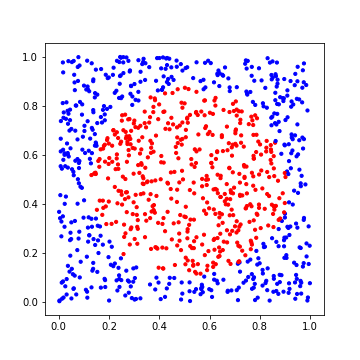
\includegraphics[scale=0.5]{../images/best_model.png}
    \caption{Predictions of the best model}
    \label{fig:best_model}
\end{figure}
\section{Summary}



\bibliographystyle{IEEEtran}
\bibliography{dl_report}

\end{document}
